


\section{What is it?}
\subsection{A little bit of history}
Before delving into the gradient descent algorithm, I recommend studying a bit of calculus,
specifically differential calculus. Now, let's take a moment to explore the history of the perceptron.\\

The perceptron, invented in 1943 by Warren McCulloch and Walter Pitts, is a fundamental concept in
artificial neural networks. In 1958, Frank Rosenblatt built the first implementation known as the "Mark 1
perceptron" at the Cornell Aeronautical Laboratory. It was initially designed as a machine for image recognition,
featuring an array of 400 photocells connected to neurons with weight updates performed by electric motors.\\

Rosenblatt's bold claims about the perceptron during a 1958 press conference sparked controversy.
The New York Times reported his statement that the perceptron was the "embryo of an electronic computer"
capable of various human-like abilities. This fueled speculation about the potential of perceptron-based
systems.\\

However, it is important to acknowledge the limitations of the perceptron. One such limitation is the
potentially slow training process, often requiring a significant number of iterations to achieve convergence.
Furthermore, the perceptron may struggle to provide accurate predictions, especially when faced with complex and
nonlinear problems. As I have demonstrated through various examples, these limitations highlight the need for
alternative neural network architectures and advanced learning algorithms to overcome these challenges and
improve prediction accuracy. It is crucial to consider these factors when applying the perceptron or exploring
other approaches in the field of artificial intelligence.

\subsection{First approach to the algorithm}
\subsubsection{How we can measure the error from our models?}
Before delving into the gradient descent algorithm, let's address the question of how to measure this error.
In our previous discussions, we derived an expression that enables us to evaluate and update the weights of
our model. This expression serves as a means to assess the discrepancy between the predicted outputs of our
model and the actual outcomes. By utilizing this error measurement, we optimize the weights
to improve the accuracy of our model.
\[
\varepsilon_t = y_t - (\vec{x}_t \cdot \vec{w}_k)
\]
However, this measurement only works for a single input and output, which is not quite useful if we want to
understand the overall accuracy of our model across the entire dataset. To address this limitation, the
first approach that comes to mind is to sum all the potential $\varepsilon_t$ values from our dataset.
\[
\sum_{t = 1}^{n}(y_t - (\vec{x}_t \cdot \vec{w}_k))
\]
The challenge with this calculation is that the resulting values can have both positive and negative signs,
which makes interpretation challenging. To address this issue, we can take the absolute value of each
$\varepsilon_t$, considering only the magnitude of the error. Additionally, we can normalize the error
by scaling it with
$\frac{1}{n}$, where $n$ represents the number of data inputs. This normalization ensures a consistent and
meaningful measure of the error.
\[
\frac{1}{n} \cdot \sum_{t = 1}^{n}|(y_t - (\vec{x}_t \cdot \vec{w}_k))|
\]
Now, this expression proves to be highly valuable in measuring the error of our model. It further emphasizes
the significance of utilizing a substantial amount of data. By incorporating a large and diverse dataset, we
can obtain more comprehensive and reliable error measurements, enhancing our understanding of the model's
performance.\\

This expression is the key to optimizing our learning algorithm for both types of neurons. As this expression
approaches zero, it indicates that we are getting closer to finding the most optimal weights. It serves as a
critical indicator of our model's performance and guides us in refining our learning process.
\[
\frac{1}{n} \cdot \sum_{t = 1}^{n}|(y_t - (\vec{x}_t \cdot \vec{w}_k))|\quad \rightarrow \quad 0
\quad \implies \quad \vec{w}_k \quad \rightarrow \quad \vec{\theta}^*
\]
It is important to remember that $\vec{\theta}^*$ represents the desired optimal weights. This expression is
commonly referred to as the \textbf{Mean Absolute Error}, which quantifies the average magnitude of the errors
in our model's predictions.
\subsubsection{How we can use this expression?}
Before diving into the details, I recommend taking some time to study calculus concepts such as derivatives, as
they
will be essential in understanding the algorithm. Now, let's proceed. We can envision the Mean Absolute Error
as a function of the weight vector $\vec{w}_k$.
\[
MAE(\vec{w}) = \frac{1}{n} \cdot \sum_{t = 1}^{n}|(y_t - (\vec{x}_t \cdot \vec{w}))|
\]
Then let me ask you a question: What is the graph representation of an absolute value function? Well, this is it.
\begin{center}
\begin{tikzpicture}[scale=1.5]
  % Axis
  \draw[->] (-2,0) -- (2,0) node[right] {$\vec{w}$};
  \draw[->] (0,-2) -- (0,2) node[above] {$MAE$};

  % Absolute value function
  \draw[domain=-2:2,smooth,variable=\x,blue] plot ({\x},{abs(\x)});
\end{tikzpicture}
\end{center}

We know that we start with random weights, and those are our initial weights $\vec{w}_0$. We can plot this
vector on our graph, which may look like this. However, it is important to note that this graph is based on
the assumption that all values of $\vec{w}$ lie along a single line.

\begin{center}
\begin{tikzpicture}[scale=1.5]
  % Axis
  \draw[->] (-2,0) -- (2,0) node[right] {$\vec{w}$};
  \draw[->] (0,-2) -- (0,2) node[above] {$MAE$};

  % Absolute value function
  \draw[domain=-2:2,smooth,variable=\x,blue] plot ({\x},{abs(\x)});

  % w0
  \draw[dashed] (-1,0) node[below] {$\vec{w}_0$} -- (-1,1);
  
  % Dot for w0
  \filldraw[red] (-1,1) circle (1pt);

  % Output of MAE(w0)
  \draw[dashed] (0,1)  -- (-1, 1) node[left] {$MAE(\vec{w}_0)$};
\end{tikzpicture}
\end{center}
From this perspective of the graph, we can clearly identify the location of the optimal weights $\vec{\theta}^*$.
\begin{center}
\begin{tikzpicture}[scale=1.5]
  % Axis
  \draw[->] (-2,0) -- (2,0) node[right] {$\vec{w}$};
  \draw[->] (0,-2) -- (0,2) node[above] {$MAE$};

  % Absolute value function
  \draw[domain=-2:2,smooth,variable=\x,blue] plot ({\x},{abs(\x)});

  % w0
  \draw[dashed] (-1,0) node[below] {$\vec{w}_0$} -- (-1,1);
  
  % Dot for w0
  \filldraw[red] (-1,1) circle (1pt);

  % Output of MAE(w0)
  \draw[dashed] (0,1)  -- (-1, 1) node[left] {$MAE(\vec{w}_0)$};
  
  \filldraw[red] (0, 0) circle (2pt) node[below right] {$\vec{\theta}^*$};
\end{tikzpicture}
\end{center}

Our final question is whether there is a way to determine the path from any random
$\vec{w}_0$ to $\vec{\theta}^*$, as it appears to be possible from this perspective. We need to identify
the direction and trajectory to reach the optimal weights.

\begin{center}
\begin{tikzpicture}[scale=1.5]
  % Axis
  \draw[->] (-2,0) -- (2,0) node[right] {$\vec{w}$};
  \draw[->] (0,-2) -- (0,2) node[above] {$MAE$};

  % Absolute value function
  \draw[domain=-2:2,smooth,variable=\x,blue] plot ({\x},{abs(\x)});

  % w0
  \draw[dashed] (-1,0) node[below] {$\vec{w}_0$} -- (-1,1);
  
  % Dot for w0
  \filldraw[red] (-1,1) circle (1pt);

  % Output of MAE(w0)
  \draw[dashed] (0,1)  -- (-1, 1) node[left] {$MAE(\vec{w}_0)$};
  
  \filldraw[red] (0, 0) circle (2pt) node[below right] {$\vec{\theta}^*$};

  % Arrow from w0 to Theta*
  \draw[->, red] (-1, -0.4) -- (-0.1, -0.4);
\end{tikzpicture}
\end{center}
The answer to that question is the gradient descent algorithm. Gradient descent is an optimization algorithm
that, given a function, not only finds a direction towards its local minimum value but also determines a better
proportion for the updates. In our example, the local minimum value corresponds to $\vec{\theta}^*$. By following
the direction and proportion
indicated by the gradient descent algorithm, we update our weights, consistently moving towards the
local minimum position. This is the fundamental concept behind the algorithm.

\section{Diving into the algorithm}
\label{sec:diving_into_the_algorithm}
direction and magnitude of weight adjustments? This was the final question we addressed in the previous
section. The solution lies within the gradient descent algorithm, but how does it solve it? It is solved by
utilizing the realm of calculus. Through calculus, we can optimize our approach by identifying the minimum
and maximum points of a function. If you have completed the homework assigned at the beginning of this
chapter, you will grasp the concept that the derivative of a function at a specific point represents the
rate of change of that function, which makes sense because the notation of derivatives, introduced by
Gottfried Wilhelm Leibniz, represents a fraction or a rate.
\[
\frac{d}{dx}(f(x)) = \lim_{h \rightarrow 0}\frac{f(x + h) - f(x)}{h}
\]
Then, I have been withholding something that you might have already noticed if you studied as I suggested
earlier. The absolute function, $f(x) = |x|$, is not a differentiable function, which poses a challenge when
using calculus in our approach. To leverage calculus effectively, we require differentiable functions that
exhibit continuity. The absolute value function lacks continuity at $x \rightarrow 0$, so it is not
usefull.\\

Fortunately, there is an alternative approach. By replacing the absolute value function with a second-degree
polynomial, we can achieve a similar effect. This modified expression is known as the Mean Square Error. With
the Mean Square Error, we address the issue of continuity and arrive at our algorithm.
\[
MSE(\vec{w}) = \frac{1}{n} \cdot \sum_{t = 1}^{n}(y_t - (\vec{x}_t \cdot \vec{w}))^2
\]
The graph of this function would resemble something like this, considering the perspective of $\vec{w}$
as a single variable.
\begin{center}
\begin{tikzpicture}[scale=1.5]
  % Axis
  \draw[->] (-2,0) -- (2,0) node[right] {$\vec{w}$};
  \draw[->] (0,-2) -- (0,4) node[above] {$MSE$};

  % Square function
  \draw[domain=-2:2,smooth,variable=\x,blue] plot ({\x},{\x*\x});

  % w0
  \draw[dashed] (-1,0) node[below] {$\vec{w}_0$} -- (-1,1);
  
  % Dot for w0
  \filldraw[red] (-1,1) circle (1pt);

  % Output of MSE(w0)
  \draw[dashed] (0,1)  -- (-1, 1) node[left] {$MSE(\vec{w}_0)$};
  
  \filldraw[red] (0, 0) circle (2pt) node[below right] {$\vec{\theta}^*$};
\end{tikzpicture}
\end{center}

This approach is immensely valuable as it provides us with information regarding the direction in which to
move and the appropriate magnitude of weight updates. Consider this logical reasoning: the derivative guides
us towards optimal weight adjustments, enabling us to make informed decisions about how much to modify the
weights. Let's follow the next example: We want to iteratively find the minimum value of that function.

\[
f(x) = x^2,\quad x_0 = 5
\]

\[
\frac{d(f(x))}{dx}(x_0) = 2 \cdot x_0 = 10 > 0
\]
Here I define my learning reate $\gamma$.
\[
\gamma = 0.1
\]
Notice that I'm subtracting the value of the derivative multiplied by the learning rate $\gamma$.
\[
x_1 = x_0 - \gamma * \frac{d(f(x))}{dx}(x_0) = 5 - 0.1 = 4.9
\]
Then, if we repeat this process until $n = 100$, we will obtain results like these.
\[
x_{100} = 1.0185179881672439\cdot10^{-9} = 0.0000000010185179881672439
\]
Generally, that is the basic idea behind the gradient descent algorithm. However, it's not as straightforward
as it seems. Since our function takes a vector $\vec{w}$ as an input, traditional derivatives for abstract
vectors do not exist. Instead, we utilize partial derivatives, denoted as $\frac{\partial f}{\partial x_1}$,
to approximate the concept. Another important concept is the gradient, represented by the nabla symbol
($\nabla$), which encompasses the partial derivatives in vector form.
\[
\nabla MSE(\vec{w}) =
\begin{bmatrix} \frac{\partial MSE}{\partial w_1}(\vec{w})
  \\ \vdots
  \\ \frac{\partial MSE}{\partial w_m}(\vec{w})
\end{bmatrix}
\]
This is where things start to get more complex. I recommend studying calculus, specifically the chain rule,
as we will be using it. When all components of the gradient approach zero,
$\nabla MSE(\vec{w}) = [0, \cdots, 0]$, we have found our desired vector of weights, $\vec{\theta}^*$.
Graphically, it may look like this.

\begin{center}
\begin{tikzpicture}
\begin{axis}[
  xlabel=$\vec{w}$,
  ylabel=$MSE(\vec{w})$,
  xmin=-5,xmax=5,
  ymin=-1,ymax=10,
  axis lines=center,
  domain=-3:3,
  samples=100,
  xtick=\empty, % removes numbers from x-axis
  ytick=\empty, % removes numbers from y-axis
]
\addplot+[mark=none] {x^2+2};
\node[label={below left:$\vec{\theta}^*$}, circle, fill, inner sep = 2pt, red] at (axis cs:0,0) {};
\draw[thick] (250, 30) -- (750, 30);
\node[label={below left:$\scriptstyle \nabla MSE(\vec{\theta}^*) = [0, \cdots, 0]$}] at (axis cs:0,2) {};
\end{axis}
\end{tikzpicture}
\end{center}

Utilizing each of these partial differences as finite differences enables us to cover all the components of
the gradient descent algorithm. However, let's delve deeper into these concepts and explore the gradient
descent method more thoroughly. To begin, let's revisit the meaning of $\vec{x}_t \cdot \vec{w}$, which
represents the dot product between $\vec{x}_t$ and $\vec{w}$.
\[
\vec{x}_t \cdot \vec{w} = \sum_{i = 1}^{m} x_{t, i} \cdot w_i = (x_{t, 1} \cdot w_1 + \cdots + x_{t, m} \cdot w_m)
\]
Where $m$ is the number of components that each vector has, so if we replace this into our definition
$MSE(\vec{w})$ we could arrive to this expression.
\[
MSE(\vec{w}) = \frac{1}{n} \cdot \sum_{t = 1}^{n}(y_t - \sum_{i = 1}^{m}x_{t, i} \cdot w_i)^2
= \frac{1}{n} \cdot ((y_1 - \sum_{i = 1}^{m}x_{1, i} \cdot w_i)^2 + \cdots + (y_n - \sum_{i = 1}^{m}x_{n, i} \cdot w_i)^2)
\]
To avoid the need for finite differences and arrive at a more concise expression, we can leverage the
chain rule. For instance, we can define.
\[
u_t = y_t - \vec{x}_t \cdot \vec{w} = y_t - \sum_{i = 1}^{m}x_{t, i} \cdot w_i
= y_t - (x_{t, 1} \cdot w_1 + \cdots + x_{t, m} \cdot w_m)
\]
If we take the partial derivative of any $u_t$ with respect to $m_i$, it is referred to as a partial derivative
because we can think of $u_t$ as a multivariable function $u_t(\vec{w})$.
\[
\frac{\partial u_t}{\partial w_i} = x_{t, i}
\]
By making this simple substitution, we can calculate the partial derivative of $w_i$ in $MSE(\vec{w})$.
\[
\frac{\partial MSE}{\partial w_i} = \frac{1}{n} \cdot (
\frac{\partial (y_1 - \vec{x}_1 \cdot \vec{w})^2}{\partial w_i} + \cdots +
\frac{\partial (y_n - \vec{x}_n \cdot \vec{w})^2}{\partial w_i})
\]

By applying the chain rule, we can easily obtain the partial derivatives.
\[
\frac{\partial MSE}{\partial w_i} = \frac{1}{n} \cdot (
\frac{\partial u_1^2}{\partial u_1} \cdot \frac{\partial u_1}{\partial w_i} + \cdots +
\frac{\partial u_n^2}{\partial u_n} \cdot \frac{\partial u_n}{\partial w_i})
\]

\[
\frac{\partial MSE}{\partial w_i} = \frac{1}{n} \cdot (
2 \cdot u_1 \cdot x_{1, i} + \cdots +
2 \cdot u_n \cdot x_{n, i})
\]

\[
\frac{\partial MSE}{\partial w_i} = \frac{1}{n} \cdot (
2 \cdot (y_1 - \vec{x}_1 \cdot \vec{w}) \cdot x_{1, i} + \cdots +
2 \cdot (y_n - \vec{x}_n \cdot \vec{w}) \cdot x_{n, i})
\]
In the end, we arrive at this simple formula, which allows us to update each of the weights.
\[
\frac{\partial MSE}{\partial w_i} = \frac{2}{n} \cdot \sum_{t = 1}^n(y_t - \vec{x}_t \cdot \vec{w}) \cdot x_{t, i}
\]
And if you know more mathematics you could adapt and modify this expression as your convinient,
for the moment we can be able to compute our gradient.
\[
\nabla MSE(\vec{w}) =
\begin{bmatrix} \frac{\partial MSE}{\partial w_1}(w_1)
  \\ \vdots
  \\ \frac{\partial MSE}{\partial w_m}(w_m)
\end{bmatrix} =
\begin{bmatrix} \frac{2}{n} \cdot \sum_{t = 1}^n(y_t - \vec{x}_t \cdot \vec{w}) \cdot x_{t, 1}
  \\ \vdots
  \\ \frac{2}{n} \cdot \sum_{t = 1}^n(y_t - \vec{x}_t \cdot \vec{w}) \cdot x_{t, m}
\end{bmatrix} 
\]
Using this gradient, we can update our weights by subtracting. As you can see, this new algorithm is not easy
to understand without a mathematical background. It requires mathematical knowledge to appreciate its efficiency.
\[
\vec{w}_{k + 1} = \vec{w}_k + \gamma \cdot \nabla MSE(\vec{w_k})
\]
Notice that I'm using addition instead of subtraction here as previously explained in this
\hyperref[sec:diving_into_the_algorithm]{example}.
The reason for this choice is that the expression $y_t - \vec{x}_t \cdot \vec{w}_k$
can be either negative or positive, representing different concepts or conditions.
\[
\frac{2}{n} \cdot \sum_{t = 1}^n(y_t - \vec{x}_t \cdot \vec{w}_k) \cdot x_{t, i} < 0\quad \implies \quad
\text{Decrement}
\]

\[
\frac{2}{n} \cdot \sum_{t = 1}^n(y_t - \vec{x}_t \cdot \vec{w}_k) \cdot x_{t, i} > 0 \quad \implies \quad
\text{Increament}
\]
So, by using a negative sign instead of moving towards $\vec{\theta}^*$, we will move in the opposite direction.
If you prefer to use a negative sign, you can multiply the entire expression of $\nabla MSE(\vec{w})$ by $-1$.
\[
(-1) \cdot \nabla MSE(\vec{w}) = \begin{bmatrix} (-1) \cdot \frac{\partial MSE}{\partial w_1}(w_1)
  \\ \vdots
  \\ (-1) \cdot \frac{\partial MSE}{\partial w_m}(w_m)
\end{bmatrix} =
\begin{bmatrix} \frac{2}{n} \cdot \sum_{t = 1}^n(\vec{x}_t \cdot \vec{w} - y_t) \cdot x_{t, 1}
  \\ \vdots
  \\ \frac{2}{n} \cdot \sum_{t = 1}^n(\vec{x}_t \cdot \vec{w} - y_t) \cdot x_{t, m}
\end{bmatrix} 
\]

\subsection{How to use it into the classification neuron?}
There is something I haven't mentioned yet. The entire gradient descent algorithm seems suitable for prediction
neurons, but how can we apply it to classification neurons? In the previous chapters, we described
classification neurons that use the activation function sign. However, using such those activation functions
causes
information loss, and it also prevents the derivative calculation due to the lack of continuity.
This is where we can employ another classic function called the sigmoid function.
\begin{figure}[H]
  \centering
  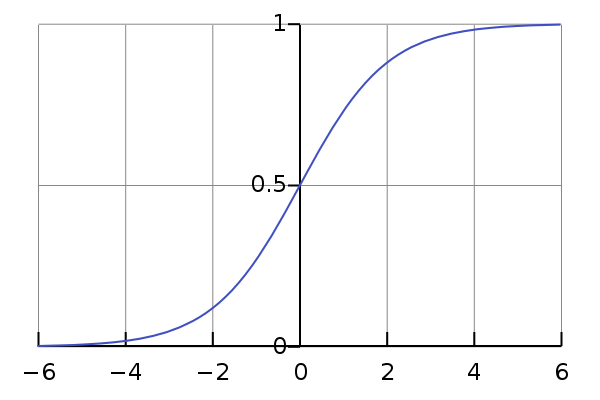
\includegraphics[scale = 0.4]{Logistic-curve.png}
  \caption{Sigmoid function}
\end{figure}

\subsubsection{Whats sigmoid function?}
A sigmoid function refers to a mathematical function that is bounded, differentiable, and defined for all real
input values. It exhibits a characteristic "S"-shaped curve and has a non-negative derivative at every point.
It is important to note that the terms "sigmoid function" and "sigmoid curve" refer to the same mathematical
object. which is defined by the formula:
\[
S(x) = \frac{1}{1 + e^{-x}} = \frac{e^x}{e^x + 1} = 1 - S(-x)
\]
This expression provides us with the following information.
\[
x \rightarrow \infty \quad \implies \quad S(x) = \frac{1}{1 + e^{-x}} \rightarrow 1
\]
\[
x \rightarrow  - \infty \quad \implies \quad S(x) = \frac{1}{1 + e^{-x}} \rightarrow 0
\]
Which fits perfectly as a solution to our problem.
\subsection{Using MSE for classification}
This concept may not be intuitively clear, but it effectively measures the error of the neuron.
Therefore, the function $MSE$ designed for classification tasks should resemble the following form.
\[
MSE(\vec{w}) = \frac{1}{n} \cdot \sum_{t = 1}^{n}(y_t - \frac{1}{1 + e^{-(\vec{x}_t \cdot \vec{w})}})^2
\]
Building upon the previous concept of gradient descent, we can derive these formulas. I understand that
this may seem challenging, but studying calculus and revisiting these ideas will enable you to comprehend
how these algorithms function.\\
Again first lets define our $u_t$

\[
u_t = y_t - \frac{1}{1 + e^{-(\vec{x}_t \cdot \vec{w})}} = y_t - \frac{1}{1 + e^{-(\sum_{i = 1}^m x_{t, i} \cdot w_i)}}
= y_t - \frac{1}{1 + e^{-x_{t, 1} \cdot w_1} \cdots e^{-x_{t, m} \cdot w_m}}
\]

Finding the derivative of $w_i$ in this case is not straightforward due to the presence of a fraction and
the Euler exponential. However, by following the fundamental rules of derivatives, we can tackle this challenge.

\[
f(x) = \frac{g(x)}{h(x)}
\]

\[
\frac{d(f(x))}{dx} = \frac{\frac{d(g(x))}{dx} \cdot h(x) - \frac{d(h(x))}{dx} \cdot g(x)}{h^2(x)}
\]

\[
f(x) = c_1 \cdot e^{c_2 \cdot x}
\]

\[
\frac{d(f(x))}{dx} = c_1 \cdot c_2 \cdot e^{c_2 \cdot x}
\]

Folling those rules we arrive with this idea of the derivate $u_t$ of $w_i$, lets view.
\[
u_t(\vec{w}) = \frac{g(\vec{w})}{h(\vec{w})}
\]

\[
g(\vec{w}) = 1
\]

\[
h(\vec{w}) = 1 + e^{-(\vec{x}_t \cdot \vec{w})} = 1 + e^{-(\sum_{i = 1}^m x_{t, i} \cdot w_i)}
= 1 + e^{-x_{t, 1} \cdot w_1} \cdots e^{-x_{t, m} \cdot w_m}
\]

\[
\frac{\partial g(\vec{w})}{\partial w_i} = 0
\]

\[
\frac{\partial h(\vec{w})}{\partial w_i}
= -x_{t, i} \cdot e^{-x_{t, 1} \cdot w_1} \cdots e^{-x_{t, i} \cdot w_i} \cdots e^{-x_{t, m} \cdot w_m}
\]

\[
\frac{\partial u_t}{\partial w_i} =
\frac{- (-x_{t, i} \cdot e^{-x_{t, 1} \cdot w_1} \cdots e^{-x_{t, i} \cdot w_i} \cdots e^{-x_{t, m} \cdot w_m})}
     {(1 + e^{-x_{t, 1} \cdot w_1} \cdots e^{-x_{t, m} \cdot w_m})^2}
     \]
     \[
     = \frac{x_{t, i} \cdot e^{-x_{t, 1} \cdot w_1} \cdots e^{-x_{t, i} \cdot w_i} \cdots e^{-x_{t, m} \cdot w_m}}
     {1 + 2e^{-x_{t, 1} \cdot w_1} \cdots e^{-x_{t, m} \cdot w_m} + e^{-2 \cdot x_{t, 1} \cdot w_1} \cdots e^{-2 \cdot x_{t, m} \cdot w_m}}
\]
I understand that these types of derivatives can be challenging to grasp, but by studying
differential calculus, you will be able to overcome the difficulties and comprehend them.

\[
\frac{\partial u_t}{\partial w_i} =
\frac{x_{t, i} \cdot e^{- \vec{x}_t \cdot \vec{w}}}
     {(1 + e^{- \vec{x}_t \cdot \vec{w}})^2}
\]

Continuing with the chain rule, we can arrive at these expressions.
\[
\frac{\partial MSE}{\partial w_i} = \frac{1}{n} \cdot (\frac{\partial u_1^2}{\partial u_1} \cdot
\frac{u_1}{w_i} + \cdots + \frac{\partial u_n^2}{\partial u_n} \cdot \frac{\partial u_n}{\partial w_i})
\]


\[
\frac{\partial MSE}{\partial w_i} = \frac{1}{n} \cdot (2 \cdot u_1 \cdot
\frac{x_{1, i} \cdot e^{- \vec{x}_1 \cdot \vec{w}}}{(1 + e^{- \vec{x}_1 \cdot \vec{w}})^2}
+ \cdots +
2 \cdot u_n \cdot
\frac{x_{n, i} \cdot e^{- \vec{x}_n \cdot \vec{w}}}{(1 + e^{- \vec{x}_n \cdot \vec{w}})^2}
\]

\[
\frac{\partial MSE}{\partial w_i} = \frac{2}{n} \cdot (
(y_1 - \frac{1}{1 + e^{-(\vec{x}_1 \cdot \vec{w})}}) \cdot
\frac{x_{1, i} \cdot e^{- \vec{x}_1 \cdot \vec{w}}}{(1 + e^{- \vec{x}_1 \cdot \vec{w}})^2}
+ \cdots +
(y_n - \frac{1}{1 + e^{-(\vec{x}_n \cdot \vec{w})}}) \cdot
\frac{x_{n, i} \cdot e^{- \vec{x}_n \cdot \vec{w}}}{(1 + e^{- \vec{x}_n \cdot \vec{w}})^2}
)
\]


\[
\frac{\partial MSE}{\partial w_i} = \frac{2}{n} \cdot \sum_{t = 1}^n
(y_t - \frac{1}{1 + e^{-\vec{x}_t \cdot \vec{w}}}) \cdot
\frac{x_{t, i} \cdot e^{- \vec{x}_t \cdot \vec{w}}}{(1 + e^{- \vec{x}_t \cdot \vec{w}})^2}
\]

And that's it! By finding the gradient, we can now implement the gradient descent algorithm
for neuron classification.
\[
\nabla MSE(\vec{w}) =
\begin{bmatrix} \frac{\partial MSE}{\partial w_1}(\vec{w})
  \\ \vdots
  \\ \frac{\partial MSE}{\partial w_m}(\vec{w})
\end{bmatrix} =
\begin{bmatrix} \frac{2}{n} \cdot \sum_{t = 1}^n
  (y_t - \frac{1}{1 + e^{-(\vec{x}_t \cdot \vec{w})}}) \cdot
  \frac{x_{t, 1} \cdot e^{- \vec{x}_t \cdot \vec{w}}}{(1 + e^{- \vec{x}_t \cdot \vec{w}})^2}
  \\ \vdots
  \\ \frac{2}{n} \cdot \sum_{t = 1}^n  (y_t - \frac{1}{1 + e^{-(\vec{x}_t \cdot \vec{w})}}) \cdot
  \frac{x_{t, m} \cdot e^{- \vec{x}_t \cdot \vec{w}}}{(1 + e^{- \vec{x}_t \cdot \vec{w}})^2}
\end{bmatrix}
\]

\[
\vec{w}_{k + 1} = \vec{w}_{k} + \gamma \cdot \nabla MSE(\vec{w}_k)
\]

\subsubsection{The Origin of the Name "Gradient Descent"}
Essentially, the name "gradient descent" derives from the concept of descending along the gradient of a
parabolic graph, as demonstrated earlier. As the weights are updated, they gradually move downwards,
resembling a descent. The following illustration depicts this idea, with each node representing a weight update.
\begin{figure}[H]
  \centering
  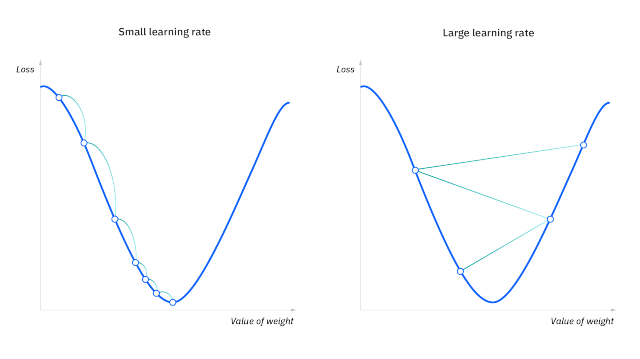
\includegraphics[scale = 0.7]{gradient_descent.png}
  \caption{Gradient descent}
\end{figure}

\section{From algorithm to code}
In this section, we will learn how to code the new optimized learning algorithm for both prediction
and classification neurons, then. When it comes to dealing with derivatives, there are different approaches
available.
One common method is to approximate the derivatives of a function using numerical techniques such as
finite differences. This method is relatively straightforward and relies on the concept of derivatives.
In the case of a multivariable function, the approximation would look something like this.


\[
\frac{\partial (f(\vec{x}))}{\partial x_i} \approx \frac{f(x_1, \cdots, x_i + h, \cdots, x_n) -
  f(x_1, \cdots, x_i, \cdots, x_n)}{h}
\]

Here, the parameter $h$ is not constrained by any specific limit. It represents your choice of
approximation, allowing you to determine the desired level of precision for the approximation.\\

However, in our case, we have derived and arrived at useful mathematical expressions
for both prediction and classification in the previous section so we are going to use it.

\subsection{Coding the Optimized Learning Algorithm for the Prediction Neuron}
So the algorithm doesn't change much. Let's begin by coding our $MSE(\vec{w})$ function to measure
the error of our model.
\[
MSE(\vec{w}) = \frac{1}{n} \cdot \sum_{t = 1}^ny_t - \vec{x}_t \cdot \vec{w}
\]

The code translation of this would look something like the following.
\begin{verbatim}
diffs = 0.0
for (t = 0, t < n, t++)
    res = 0.0
    for (i = 0, i < input[t].size(), i++)
        res += (inputst[t][i] * weigths[i])
    diffs += pow(outputs[t] - res, 2.0)  // Compute the square

return  diffs / n
\end{verbatim}
With this code written as a function, we now have the ability to measure the performance of our model.
As for the learning algnnorithm, as I mentioned earlier, the new algorithm for updating our weights doesn't
need to change much. You only need to keep in mind this expression.
\[
\frac{\partial MSE}{\partial w_i} = \frac{2}{n} \cdot \sum_{t = 1}^n(y_t - \vec{x}_t \cdot \vec{w}) \cdot x_{t, i}
\]
First define your number of epochs, and learning rate which is gamma $\gamma$.
\begin{verbatim}
gamma = 0.1
nepochs = 100
\end{verbatim}
Now, let's proceed with coding the algorithm. Since this algorithm iteratively works by summing values,
there are multiple approaches to achieve the same result. Hence, the following implementation is not the
only way to do it.
\begin{verbatim}
for (e = 0, e < nepochs, e++)
    errors[n] = {0.0}
    // First compued the whole errors
    for (t = 0, t < n, t++)
        res = 0.0
        for (i = 0, i < input[t].size(), i++)
            res += inputst[t][i] * weigths[i]
        errors[t] = outputs[t] - res

    // After update all the weights
    for (i = 0, i < weights.size(), i++)
        update = 0.0
        for (t = 0, t < n, t++)
            update += errors[t] * input[t][i]
        weights[i] += (2 / n) * gamma * update
\end{verbatim}

\subsection{Coding the Optimized Learning Algorithm for the Classification Neuron}
Now, let's begin implementing the algorithm for the classification neuron. The first step is to code
the sigmoid function activation, which is essential for our computations.
\begin{verbatim}
function activation(x)
         return 1 / (1 + exp(- x))
end function
\end{verbatim}
ost programming languages have a built-in function called $exp$ that represents the exponential function $e^x$.
With this function, we can proceed to code our own $MSE$ function to assess the accuracy of our model.
\[
MSE(\vec{w}) = \frac{1}{n} \cdot \sum_{t = 1}^{n}(y_t - \frac{1}{1 + e^{-(\vec{x}_t \cdot \vec{w})}})^2
\]
\begin{verbatim}
diffs = 0.0
for (t = 0, t < n, t++)
    res = 0.0
    for (i = 0, i < input[t].size(), i++)
        res += inputst[t][i] * weigths[i]
    diffs += pow(outputs[t] - activation(res), 2.0) // notice that I call activation

return  diffs / n
\end{verbatim}
The learning algorithm for the classification neuron is slightly different, as we introduce the sigmoid
function and incorporate new expressions into it. As a result, the code would look like the following,
but just try to follow this expression.
\[
\frac{\partial MSE}{\partial w_i} = \frac{2}{n} \cdot \sum_{t = 1}^n
(y_t - \frac{1}{1 + e^{-\vec{x}_t \cdot \vec{w}}}) \cdot
\frac{x_{t, i} \cdot e^{- \vec{x}_t \cdot \vec{w}}}{(1 + e^{- \vec{x}_t \cdot \vec{w}})^2}
\]

I hope you have understood this code. If you find it challenging to comprehend, I recommend trying to write
your own algorithm and then revisiting this code. My approach aims to minimize computations for improved
efficiency, and I believe there is room for further optimization.
\begin{verbatim}
for (e = 0, e < nepochs, e++)
    errors[n] = {0.0}
    // Notice that I'm creating this array to save computations
    results[n] = {0.0}
    // First compued the whole errors
    for (t = 0, t < n, t++)
        res = 0.0
        for (i = 0, i < input[t].size(), i++)
            res += inputs[t][i] * weigths[i]
        results[t] = res
        errors[t] = outputs[t] - activation(res)

    // After update all the weights
    for (i = 0, i < weights.size(), i++)
        update = 0.0
        for (t = 0, t < n, t++)
            update += errors[t] * pow(activation(results[t]), 2.0)
                      * inputs[t][i] * exp(- results[t])
        weights[i] += (2 / n) * gamma * update
\end{verbatim}
You might be wondering about the feed-forward code, but I believe it is unnecessary to
show it here since it is practically the same code we have written in the previous chapter.
\section{Examples}
I have created a Fortran module that supports both types of neurons. After implementing the module,
I have organized illustrative examples that you can explore in the following link:
\href{https://github.com/alecksandr26/fortran-ml/tree/main/examples}{examples}.
Feel free to check
them out while you continue reading this section.
\subsection{Fortran module for both type of neurons}
As mentioned earlier, I designed the module to support both types of neurons, aiming for a more generalized
approach. This allows for code reusability across various problem domains. By adopting this design, we can
leverage the module for a wide range of applications, this is the link for the following code:
\hyperrf{}{}.

\begin{lstlisting}

\end{lstlisting}




